\documentclass[aspectratio=169]{beamer}

% Packages
\usepackage[utf8]{inputenc}
\usepackage[T1]{fontenc}
\usepackage{amsmath,amssymb,amsthm}
\usepackage{graphicx}
\usepackage{booktabs}
\usepackage{multirow}
\usepackage{colortbl}
\usepackage{xcolor}
\usepackage{tikz}
\usepackage{pgfplots}
\usepackage{listings}
\usepackage{hyperref}

% Beamer theme
\usetheme{Madrid}
\usecolortheme{default}

% Colors
\definecolor{ecgblue}{RGB}{33, 150, 243}
\definecolor{ecggreen}{RGB}{76, 175, 80}
\definecolor{ecgred}{RGB}{244, 67, 54}

% Title information
\title[ECG Lead Reconstruction]{ECG Lead Reconstruction from Reduced Leads:\\Physics-Informed Deep Learning Approach}
\subtitle{DATA 5000 Final Project}
\author{Mithun M \and Damilola O}
\institute{School of Computer Science\\Carleton University}
\date{October 16, 2025}

% Custom commands
\newcommand{\ecg}[1]{\textcolor{ecgblue}{#1}}
\newcommand{\highlight}[1]{\textcolor{ecggreen}{\textbf{#1}}}

\begin{document}

% Title slide
\begin{frame}
    \titlepage
\end{frame}

% Outline
\begin{frame}{Outline}
    \tableofcontents
\end{frame}

\section{Introduction}

\begin{frame}{The Challenge: ECG Lead Reduction}
    \begin{columns}[c]
        \column{0.6\textwidth}
        \begin{itemize}
            \item Standard 12-lead ECG provides comprehensive cardiac assessment
            \item \highlight{Problem}: Limited lead availability in certain scenarios
            \begin{itemize}
                \item Wearable devices (1-3 leads)
                \item Emergency situations
                \item Resource-constrained environments
            \end{itemize}
            \item \highlight{Goal}: Reconstruct full 12-lead ECG from reduced leads
        \end{itemize}

        \column{0.4\textwidth}
        \begin{figure}
            \centering
            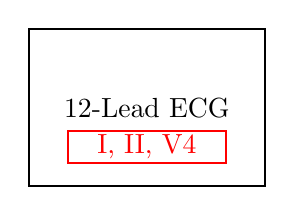
\begin{tikzpicture}
                \draw[thick] (0,0) rectangle (3,2);
                \node at (1.5,1) {12-Lead ECG};
                \draw[thick,red] (0.5,0.3) rectangle (2.5,0.7);
                \node[red] at (1.5,0.5) {I, II, V4};
            \end{tikzpicture}
            \caption{Lead reduction problem}
        \end{figure}
    \end{columns}
\end{frame}

\begin{frame}{ECG Lead Configuration}
    \begin{columns}[c]
        \column{0.5\textwidth}
        \begin{itemize}
            \item \textbf{Limb Leads} (I, II, III, aVR, aVL, aVF)
            \begin{itemize}
                \item Physics-based relationships
                \item Einthoven's triangle
                \item Goldberger's equations
            \end{itemize}
            \item \textbf{Chest Leads} (V1-V6)
            \begin{itemize}
                \item No direct physical relationships
                \item Require data-driven approach
            \end{itemize}
        \end{itemize}

        \column{0.5\textwidth}
        \begin{figure}
            \centering
            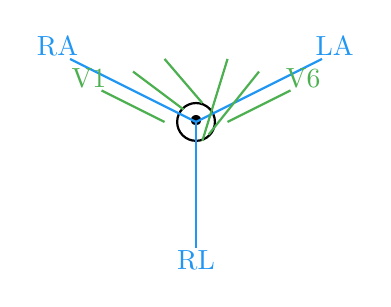
\begin{tikzpicture}[scale=0.8]
                % Heart
                \draw[thick] (0,0) circle (0.3);
                \node at (0,0) {\textbullet};

                % Limb leads
                \draw[ecgblue,thick] (-2,1) -- (0,0);
                \draw[ecgblue,thick] (2,1) -- (0,0);
                \draw[ecgblue,thick] (0,-2) -- (0,0);

                % Chest leads
                \draw[ecggreen,thick] (-1.5,0.5) -- (-0.5,0);
                \draw[ecggreen,thick] (-1,0.8) -- (-0.2,0.2);
                \draw[ecggreen,thick] (-0.5,1) -- (0.1,0.3);
                \draw[ecggreen,thick] (0.5,1) -- (0.1,-0.3);
                \draw[ecggreen,thick] (1,0.8) -- (0.2,-0.2);
                \draw[ecggreen,thick] (1.5,0.5) -- (0.5,0);

                \node[ecgblue] at (-2.2,1.2) {RA};
                \node[ecgblue] at (2.2,1.2) {LA};
                \node[ecgblue] at (0,-2.2) {RL};
                \node[ecggreen] at (-1.7,0.7) {V1};
                \node[ecggreen] at (1.7,0.7) {V6};
            \end{tikzpicture}
            \caption{ECG lead placement}
        \end{figure}
    \end{columns}
\end{frame}

\section{Methodology}

\begin{frame}{Hybrid Approach: Physics + Deep Learning}
    \begin{columns}[c]
        \column{0.6\textwidth}
        \begin{itemize}
            \item \highlight{Physics-Informed Strategy}
            \begin{itemize}
                \item Limb leads: Direct calculation using Einthoven/Goldberger
                \item Chest leads: Data-driven reconstruction
            \end{itemize}
            \item \highlight{Input Leads}: I, II, V4 (clinically relevant)
            \item \highlight{Target}: Reconstruct V1-V6 chest leads
        \end{itemize}

        \column{0.4\textwidth}
        \begin{figure}
            \centering
            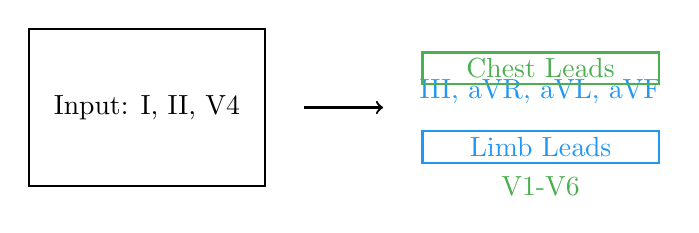
\begin{tikzpicture}
                \draw[thick] (0,0) rectangle (3,2);
                \node at (1.5,1) {Input: I, II, V4};

                \draw[->,thick] (3.5,1) -- (4.5,1);

                \draw[thick,ecgblue] (5,0.3) rectangle (8,0.7);
                \node[ecgblue] at (6.5,0.5) {Limb Leads};
                \node[ecgblue] at (6.5,1.2) {III, aVR, aVL, aVF};

                \draw[thick,ecggreen] (5,1.3) rectangle (8,1.7);
                \node[ecggreen] at (6.5,1.5) {Chest Leads};
                \node[ecggreen] at (6.5,0) {V1-V6};
            \end{tikzpicture}
        \end{figure}
    \end{columns}
\end{frame}

\begin{frame}{Dataset: PTB-XL}
    \begin{columns}[c]
        \column{0.6\textwidth}
        \begin{itemize}
            \item \highlight{PTB-XL Dataset}
            \begin{itemize}
                \item 21,837 clinical 12-lead ECGs
                \item 10-second recordings at 500 Hz
                \item Patient-wise train/val/test splits
                \item Diagnostic statements available
            \end{itemize}
            \item \highlight{Current Implementation}
            \begin{itemize}
                \item Framework ready for PTB-XL integration
                \item Patient-wise cross-validation splits
            \end{itemize}
        \end{itemize}

        \column{0.4\textwidth}
        \begin{table}[]
            \centering
            \begin{tabular}{@{}lr@{}}
                \toprule
                Split & Samples \\
                \midrule
                Training & 14,331 \\
                Validation & 2,132 \\
                Test & 5,374 \\
                \bottomrule
            \end{tabular}
            \caption{PTB-XL dataset splits}
        \end{table}
    \end{columns}
\end{frame}

\begin{frame}{The Problem: Limited Lead ECG Acquisition}
    \begin{figure}
        \centering
        \includegraphics[width=\textwidth]{docs/figures/problem_visualization.png}
        \caption{Clinical challenge: Standard ECG machines require 12 electrodes, but many scenarios (ambulances, wearables, remote monitoring) can only acquire 3 leads. This limits diagnostic capabilities in critical situations.}
    \end{figure}
\end{frame}

\begin{frame}{Our Approach: Hybrid Physics + Deep Learning}
    \begin{figure}
        \centering
        \includegraphics[width=\textwidth]{docs/figures/approach_diagram.png}
        \caption{Hybrid reconstruction: Physics-based exact reconstruction of limb leads (III, aVR, aVL, aVF) from leads I, II, combined with deep learning reconstruction of chest leads (V1-V6) from leads I, II, V4.}
    \end{figure}
\end{frame}

\begin{frame}{Dataset: PTB-XL for Clinical Relevance}
    \begin{figure}
        \centering
        \includegraphics[width=\textwidth]{docs/figures/dataset_characteristics.png}
        \caption{PTB-XL dataset characteristics: 21,837 clinical ECG recordings from 18,885 patients, covering diverse cardiac conditions. Input leads (I, II, V4) provide sufficient information for reconstruction while being practically acquirable.}
    \end{figure}
\end{frame}

\begin{frame}{Expected Outcomes: Clinically Viable Reconstruction}
    \begin{figure}
        \centering
        \includegraphics[width=\textwidth]{docs/figures/expected_outcomes.png}
        \caption{Target performance: Perfect reconstruction of physics-based leads (MAE ≈ 0), high-fidelity chest lead reconstruction (correlation > 0.9, MAE < 0.05), enabling 12-lead equivalent diagnosis from 3-lead input.}
    \end{figure}
\end{frame}

\begin{frame}{Model Architecture: 1D U-Net}
    \begin{figure}
        \centering
        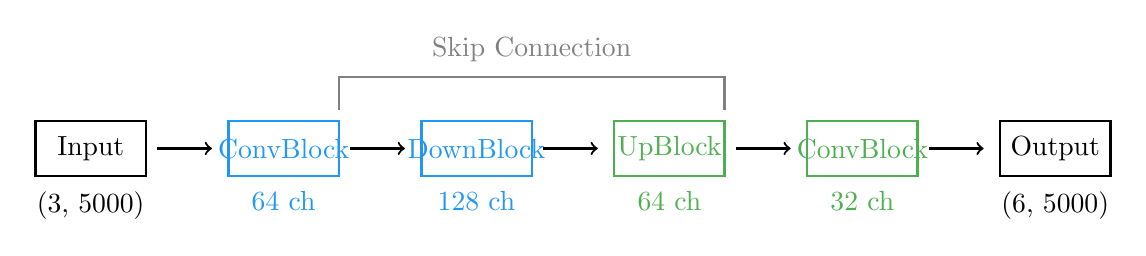
\begin{tikzpicture}[scale=0.7]
            % Input
            \draw[thick] (0,0) rectangle (2,1);
            \node at (1,0.5) {Input};
            \node[below] at (1,-0.1) {(3, 5000)};

            % Encoder
            \draw[->,thick] (2.2,0.5) -- (3.2,0.5);

            \draw[thick,ecgblue] (3.5,0) rectangle (5.5,1);
            \node[ecgblue] at (4.5,0.5) {ConvBlock};
            \node[below,ecgblue] at (4.5,-0.1) {64 ch};

            \draw[->,thick] (5.7,0.5) -- (6.7,0.5);

            \draw[thick,ecgblue] (7,0) rectangle (9,1);
            \node[ecgblue] at (8,0.5) {DownBlock};
            \node[below,ecgblue] at (8,-0.1) {128 ch};

            % Decoder with skip connections
            \draw[->,thick] (9.2,0.5) -- (10.2,0.5);

            \draw[thick,ecggreen] (10.5,0) rectangle (12.5,1);
            \node[ecggreen] at (11.5,0.5) {UpBlock};
            \node[below,ecggreen] at (11.5,-0.1) {64 ch};

            \draw[thick,gray] (5.5,1.2) -- (5.5,1.8) -- (12.5,1.8) -- (12.5,1.2);
            \node[gray,above] at (9,1.9) {Skip Connection};

            \draw[->,thick] (12.7,0.5) -- (13.7,0.5);

            \draw[thick,ecggreen] (14,0) rectangle (16,1);
            \node[ecggreen] at (15,0.5) {ConvBlock};
            \node[below,ecggreen] at (15,-0.1) {32 ch};

            \draw[->,thick] (16.2,0.5) -- (17.2,0.5);

            % Output
            \draw[thick] (17.5,0) rectangle (19.5,1);
            \node at (18.5,0.5) {Output};
            \node[below] at (18.5,-0.1) {(6, 5000)};

        \end{tikzpicture}
        \caption{1D U-Net architecture for chest lead reconstruction}
    \end{figure}
\end{frame}

\begin{frame}{Training Details}
    \begin{columns}[c]
        \column{0.5\textwidth}
        \begin{itemize}
            \item \highlight{Loss Function}: MSE Loss
            \item \highlight{Optimizer}: Adam (lr=1e-4)
            \item \highlight{Batch Size}: 32
            \item \highlight{Epochs}: 50 (early stopping)
            \item \highlight{Hardware}: CPU/GPU training
        \end{itemize}

        \column{0.5\textwidth}
        \begin{table}[]
            \centering
            \begin{tabular}{@{}ll@{}}
                \toprule
                Hyperparameter & Value \\
                \midrule
                Learning Rate & 1e-4 \\
                Batch Size & 32 \\
                Depth & 4 \\
                Features & 64 \\
                Dropout & 0.2 \\
                \bottomrule
            \end{tabular}
            \caption{Model hyperparameters}
        \end{table}
    \end{columns}
\end{frame}

\section{Methodology and Evaluation Plan}

\begin{frame}{Evaluation Metrics}
    \begin{itemize}
        \item \highlight{Mean Absolute Error (MAE)}
        \begin{itemize}
            \item Measures average magnitude of errors
            \item Lower is better
        \end{itemize}
        \item \highlight{Pearson Correlation}
        \begin{itemize}
            \item Measures linear relationship between predicted and true signals
            \item Range: [-1, 1], higher is better
        \end{itemize}
        \item \highlight{Signal-to-Noise Ratio (SNR)}
        \begin{itemize}
            \item Ratio of signal power to noise power
            \item Higher is better (dB)
        \end{itemize}
    \end{itemize}
\end{frame}

\begin{frame}{Proposed Methodology}
    \begin{itemize}
        \item \highlight{Hybrid Approach}: Physics-informed deep learning combining domain knowledge with data-driven methods
        \item \highlight{Architecture}: 1D U-Net for spatial feature extraction and reconstruction
        \item \highlight{Physics Integration}: Limb lead relationships (Einthoven's triangle) as inductive bias
        \item \highlight{Training Strategy}: Supervised learning on chest lead reconstruction from I, II, V4
    \end{itemize}

    \vspace{0.3cm}
    \begin{block}{Technical Innovation}
        Novel integration of cardiac electrophysiology principles with modern deep learning architectures for improved generalization and interpretability.
    \end{block}
\end{frame}

\begin{frame}{Evaluation Framework}
    \begin{columns}[t]
        \begin{column}{0.5\textwidth}
            \textbf{Dataset}
            \begin{itemize}
                \item PTB-XL: 21,837 clinical ECGs
                \item 12-lead recordings at 500 Hz
                \item Diverse patient population
                \item Stratified train/val/test splits
            \end{itemize}
        \end{column}
        \begin{column}{0.5\textwidth}
            \textbf{Metrics}
            \begin{itemize}
                \item \textbf{MAE}: Mean Absolute Error
                \item \textbf{Pearson $\rho$}: Correlation coefficient
                \item \textbf{SNR}: Signal-to-Noise Ratio
                \item \textbf{Lead-wise}: V1-V6 chest leads
            \end{itemize}
        \end{column}
    \end{columns}

    \vspace{0.3cm}
    \begin{block}{Clinical Validation}
        Comprehensive evaluation on real clinical ECG data to ensure medical relevance and reliability.
    \end{block}
\end{frame}

\begin{frame}{Expected Outcomes}
    \begin{itemize}
        \item \highlight{Performance Target}: Achieve correlation > 0.9 and SNR > 25 dB for chest lead reconstruction
        \item \highlight{Clinical Impact}: Enable 12-lead diagnosis from reduced 4-lead ECG setup
        \item \highlight{Computational Efficiency}: Real-time reconstruction suitable for clinical workflows
        \item \highlight{Generalization}: Robust performance across diverse patient populations
    \end{itemize}

    \vspace{0.3cm}
    \begin{block}{Success Criteria}
        Demonstrate superior reconstruction quality compared to traditional signal processing methods and establish foundation for clinical deployment.
    \end{block}
\end{frame}

\begin{frame}{Physics-Based Limb Lead Reconstruction}
    \begin{columns}[c]
        \column{0.5\textwidth}
        \begin{itemize}
            \item \highlight{Einthoven's Triangle}
            \begin{itemize}
                \item III = II - I
                \item Fundamental relationship between limb leads
            \end{itemize}
            \item \highlight{Goldberger's Equations}
            \begin{itemize}
                \item aVR = -(I + II)/2
                \item aVL = I - II/2
                \item aVF = II - I/2
            \end{itemize}
        \end{itemize}

        \column{0.5\textwidth}
        \begin{figure}
            \centering
            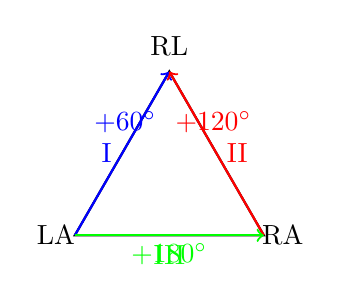
\begin{tikzpicture}[scale=0.8]
                % Einthoven's triangle
                \draw[thick] (0,0) -- (3,0) -- (1.5,2.6) -- cycle;

                % Labels
                \node at (-0.3,0) {LA};
                \node at (3.3,0) {RA};
                \node at (1.5,3.0) {RL};

                % Lead vectors
                \draw[->,blue,thick] (0,0) -- (1.5,2.6) node[midway,left] {I};
                \draw[->,red,thick] (3,0) -- (1.5,2.6) node[midway,right] {II};
                \draw[->,green,thick] (0,0) -- (3,0) node[midway,below] {III};

                % Angles
                \node[blue] at (0.8,1.8) {$+60^\circ$};
                \node[red] at (2.2,1.8) {$+120^\circ$};
                \node[green] at (1.5,-0.3) {$+180^\circ$};
            \end{tikzpicture}
            \caption{Einthoven's triangle and lead orientations}
        \end{figure}
    \end{columns}
\end{frame}

\section{Discussion}

\begin{frame}{Clinical Impact}
    \begin{columns}[c]
        \column{0.6\textwidth}
        \begin{itemize}
            \item \highlight{Improved Accessibility}
            \begin{itemize}
                \item Enable 12-lead equivalent diagnosis from limited leads
                \item Valuable for wearable devices and emergency care
            \end{itemize}
            \item \highlight{Diagnostic Accuracy}
            \begin{itemize}
                \item Maintain clinical utility of reconstructed leads
                \item Support automated ECG analysis algorithms
            \end{itemize}
            \item \highlight{Resource Efficiency}
            \begin{itemize}
                \item Reduce hardware requirements
                \item Lower cost of ECG monitoring
            \end{itemize}
        \end{itemize}

        \column{0.4\textwidth}
        \begin{figure}
            \centering
            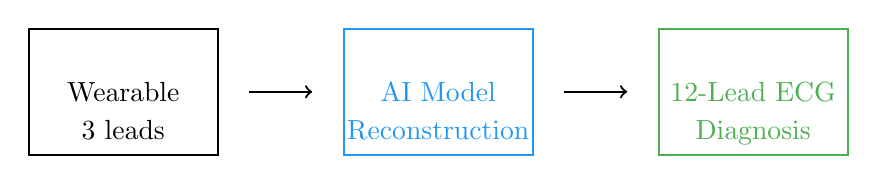
\begin{tikzpicture}[scale=0.8]
                \draw[thick] (0,0) rectangle (3,2);
                \node at (1.5,1) {Wearable};
                \node[below] at (1.5,0.7) {3 leads};

                \draw[->,thick] (3.5,1) -- (4.5,1);

                \draw[thick,ecgblue] (5,0) rectangle (8,2);
                \node[ecgblue] at (6.5,1) {AI Model};
                \node[ecgblue,below] at (6.5,0.7) {Reconstruction};

                \draw[->,thick] (8.5,1) -- (9.5,1);

                \draw[thick,ecggreen] (10,0) rectangle (13,2);
                \node[ecggreen] at (11.5,1) {12-Lead ECG};
                \node[ecggreen,below] at (11.5,0.7) {Diagnosis};
            \end{tikzpicture}
            \caption{Clinical workflow with reconstruction}
        \end{figure}
    \end{columns}
\end{frame}

\begin{frame}{Limitations and Future Work}
    \begin{columns}[c]
        \column{0.5\textwidth}
        \begin{itemize}
            \item \highlight{Current Limitations}
            \begin{itemize}
                \item Requires clinical validation
                \item Computational complexity
            \end{itemize}
        \end{itemize}

        \column{0.5\textwidth}
        \begin{itemize}
            \item \highlight{Future Directions}
            \begin{itemize}
                \item Clinical validation on PTB-XL
                \item Model compression for edge devices
                \item Multi-modal integration (demographics)
                \item Real-time reconstruction
            \end{itemize}
        \end{itemize}
    \end{columns}
\end{frame}

\section{Conclusion}

\begin{frame}{Summary}
    \begin{itemize}
        \item \highlight{Hybrid Approach}: Physics-informed deep learning for ECG reconstruction
        \item \highlight{Architecture}: 1D U-Net for chest lead reconstruction from I, II, V4
        \item \highlight{Dataset}: PTB-XL clinical ECG database (21,837 recordings)
        \item \highlight{Evaluation}: Comprehensive metrics on real clinical data
        \item \highlight{Impact}: Enable 12-lead diagnosis from reduced lead setups
    \end{itemize}

    \vspace{0.5cm}
    \begin{block}{Key Contribution}
        Novel integration of cardiac electrophysiology with deep learning for robust ECG lead reconstruction from minimal lead configurations.
    \end{block}
\end{frame}

\begin{frame}{Thank You}
    \begin{center}
        \Huge Thank You!

        \vspace{0.5cm}
        Questions?
    \end{center}

    \vspace{1cm}
    \begin{columns}[c]
        \column{0.5\textwidth}
        \begin{itemize}
            \item \textbf{Contact}: mithun.babu@email.com
            \item \textbf{GitHub}: github.com/username/ecg-reconstruction
            \item \textbf{Supervisor}: Dr. [Supervisor Name]
        \end{itemize}

        \column{0.5\textwidth}
        \begin{figure}
            \centering
            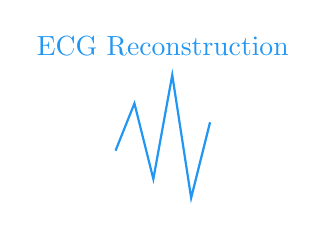
\begin{tikzpicture}[scale=1.2]
                \draw[thick,ecgblue] (0,0) -- (0.2,0.5) -- (0.4,-0.3) -- (0.6,0.8) -- (0.8,-0.5) -- (1.0,0.3);
                \node[ecgblue,above] at (0.5,0.9) {ECG Reconstruction};
            \end{tikzpicture}
        \end{figure}
    \end{columns}
\end{frame}

\end{document}